\فصل{ مفاهیم اولیه و کارهای پیشین}

در این بخش از پایان‌نامه به معرفی اجمالی مفاهیم استفاده شده می‌پردازیم.
%----------------------------- مقدمه ----------------------------------

\قسمت{هوش مصنوعی}
هوش مصنوعی یکی از جدیدترین رشته‌ها در علوم و مهندسی است و در حال حاضر طیف وسیعی از زیرشاخه‌ها (از حوزه‌های عمومی مانند یادگیری و  
\trans{ادراک}{Perception}
تا حوزه‌های خاص مانند بازی کردن شطرنج، اثبات قضایای ریاضی و …) را دربرمی‌گیرد. تعاریف مختلف و متنوعی از هوش مصنوعی وجود دارد که به‌طور کلی می‌توان آن‌ها را به چهار دسته‌ی زیر تقسیم‌بندی کرد. 
\begin{enumerate}
\item فکر کردن مانند انسان:
    \begin{itemize}
        \item خودکارسازی فعالیت‌هایی که ما با تفکر انسان مرتبط می‌کنیم. فعالیت‌هایی مانند تصمیم‌گیری، حل مسئله، یادگیری و … .        
    \end{itemize}

\item فکر کردن عقلانی:
    \begin{itemize}
        \item 
            مطالعه‌ی قوای ذهنی از طریق مدل‌های محاسباتی
        \item
            مطالعه‌ی محاسباتی که ادراک، استدلال و عمل را امکان‌پذیر می‌کند.
    \end{itemize}
    
\item عمل کردن مانند انسان:
    \begin{itemize}
        \item 
            هنر ایجاد ماشین‌هایی که کارهایی را انجام می‌دهند که وقتی توسط انسان‌ها انجام می‌شود، نیازمند هوش‌مندی است.
        \item
            مطالعه‌ی چگونگی انجام دادن کارها با کامپیوتر که در حال حاضر (سال ۱۹۹۱) انسان‌ها آن کارها را بهتر انجام می‌دهند. 
    \end{itemize}
\item عمل کردن عقلانی:
    \begin{itemize}
        \item 
        هوش محاسباتی مطالعه‌ی طراحی 
        \trans{نماینده}{agent}‌های
        هوش‌مند است.
    \end{itemize}

\end{enumerate}
\قسمت{پردازش زبان طبیعی}

پردازش زبان طبیعی به شاخه‌ای از علوم کامپیوتر، به‌طور مشخص‌تر به شاخه‌ی عمل کردن مانند انسان هوش مصنوعی که پیش‌تر به آن اشاره شد، مربوط می‌شود. این حوزه به کامپیوترها این توانایی را می‌دهد تا متن و کلمات محاوره‌ای را همان‌طور که انسان‌ها متوجه می‌شوند، بفهمند.
پردازش زبان طبیعی، زبان‌شناسی محاسباتی (
\trans{مدل‌سازی مبتنی بر قواعد زبان انسانی}{rule-based modeling of human language} 
) را با مدل‌های آماری، یادگیری ماشین و یادگیری عمیق ترکیب می‌کند. این فن‌آوری‌ها در کنار هم، کامپیوترها را قادر می‌سازند تا زبان انسان را به صورت متنی یا داده‌های صوتی پردازش کنند و معنای کامل و دقیق آن را با توجه به هدف و احساسات گوینده یا نویسنده درک کنند.
پردازش طبیعی زبان نیروی پیش‌رانه‌ی برنامه‌های کامپیوتری‌ای هستند که متن‌ها را از یک زبان به زبان دیگر ترجمه می‌کنند 
(\trans{مترجم گوگل}{Google Translate})
، به دستورات گفتاری پاسخ می‌دهند 
(\trans{مانند دستیار صوتی شرکت اپل}{Siri})
و حجم زیادی از متن را به سرعت
\trans{بی‌درنگ}{Real-Time}
) خلاصه می‌کنند. در زندگی معمولی با احتمال خوبی با کاربردهای پردازش زبان طبیعی روبه‌رو شده‌ایم. برخی از آن‌ها عبارتند از:
\begin{itemize}
    \item \trans{سیستم‌های مکان‌یاب }{GPS}
    \item دستیار‌های دیجیتال
    \item نرم‌افزارهای تبدیل گفتار به متن
    \item \trans{ربات‌های گفت‌گو}{Chat Bots}
    \item  خدمات مشتری
    \item و ...
\end{itemize}


\قسمت{وظایف پردازش زبان طبیعی}
زبان انسان مملو از ابهاماتی است که نوشتن نرم‌افزاری که به‌طور دقیق معنای متن یا داده‌های صوتی را تعیین می‌کنند، سخت می‌کند:

\begin{itemize}
    \item \trans{هم‌نام‌ها}{Homonyms}
    \item \trans{هم‌آواها}{Homophones}
    \item کنایه‌ها
    \item اصطلاحات
    \item استعاره‌ها
    \item قواعد، استثناها و تنوع در ساختار جمله
\end{itemize}
موارد بالا فقط تعداد محدودی از
\trans{بی‌نظمی‌ها}{Irregularities}ی
زبان انسان است که یادگیری آن برای انسان‌ها چندین سال طول می‌کشد اما برنامه‌نویس باید برنامه‌های کاربردی مبتنی بر زبان طبیعی را آموزش دهند تا از ابتدا به‌طور دقیق مفاهیم را شناسایی و درک کنند.
بعضی از وظایف پردازش زبان طبیعی این است که متن و داده‌های صوتی انسان را به‌طوری تقسیم‌بندی  کند تا به کامپیوترها کمک کند تا آن‌چه را که قرار است تجزیه کنند را بفهمند. برخی از این وظایف عبارتند از:
\begin{itemize}
    \item
    \textbf{تشخیص گفتار:}
    در این کاربرد، به کمک پردازش زبان طبیعی گفتار به نوشتار تبدیل می‌شود. تشخیص گفتار برای هر برنامه‌ای که از  دستورات صوتی استفاده می‌کند یا به سوالات گفتاری پاسخ می‌دهد، مورد نیاز است. چیزی که تشخیص گفتار را به‌صورت ویژه‌ای چالش‌ برانگیز می‌کند، نحوه‌ی صحبت افراد است مانند سرعت تکلم، قرینه‌های لفظی و معنوی، تاکید و لحن‌های مختلف، استفاده نادرست از قواعد زبان و ... 
    \item \textbf{برچسب‌گذاری گفتار:}
    فرآیند تشخیص بخشی از گفتار از یک کلمه یا قسمتی از متن با استفاده از نحوه‌ی استفاده از آن و زمینه است. مثلا در جمله‌ی « من این کتاب را خریدم»‌، خریدم فعل جمله است.
    \item \textbf{شناسایی موجودیت‌های نام‌گذاری‌شده:}
    کلمات یا عبارات را به عنوان موجودیت‌های مفید شناسایی می‌کند. مثلا شناسایی این که «ناجا» یک سازمان و یا «علی» نام یک مرد است را برعهده دارد.
    \item \textbf{تجزیه و تحلیل احساسات:}
    پردازش طبیعی زبان در این کاربرد سعی می‌کند تا 
    \trans{کیفیت‌های ذهنی}{Subjective Qualities}
    را از متن استخراج کند. کیفیت‌هایی ذهنی نظیر:
    \begin{itemize}
        \item نگرش‌ها
        \item احساسات
        \item کنایه
        \item سوءظن
        \item \trans{ابهامات و سردرگمی‌ها}{Confusions}
    \end{itemize}
\end{itemize}

\قسمت{پیش پردازش متن}
پیش پردازش متن یک مرحله مهم برای کارهای پردازش زبان طبیعی است. این کار متن را به شکل قابل‌هضم‌تری تبدیل می‌کند، به طوری که الگوریتم‌های یادگیری ماشین می‌توانند عملکرد بهتری داشته باشند.
به طور کلی، 3 پیش‌پردازش مهم وجود دارد:
\begin{itemize}
\item  توکن‌سازی: به طور خلاصه، توکن‌سازی در مورد تقسیم رشته‌های متن به قطعات کوچکتر یا "توکن" است. پاراگراف‌ها را می‌توان به جملات و جملات را می‌توان به کلمات تبدیل کرد.
\item نرمال‌سازی: هدف نرمال‌سازی این است که همه متن را در یک سطح بازی برابر قرار دهد، به عنوان مثال، تبدیل همه کاراکترها به حروف کوچک. 
\item حذف نویز: حذف نویز متن را پاک می‌کند، به عنوان مثال، فضاهای سفید اضافی را حذف می‌کند.
\end{itemize}


در زیر به چند مفهوم معروف پیش پردازش اشاره می‌کنیم.
\subsection{\trans{یافتن ریشه کلمات}{Lemmatization or Stemming }}
در پیش‌پردازش کلمات را به ریشه اصلی خود برمی‌گردانیم. یا حروف اضافه را از آن‌ها حذف می‌کنیم 
ریشه‌یابی یک ابتکاری است که انتها(یا بخشی از) کلمات را بریده و بنابراین، ممکن است کلمات خوب یا واقعی نباشند.


\subsection{\trans{ایست‌واژه}{Stopword}}
کلمات کلیدی کلمات بسیار متداول در هر زبان هستند. برای مثال در فارسی حروف ربط، افعال پرتکرار مانند 
"است"
و بسیاری دیگر از کلمات جزو ایست‌واژه‌ها محسوب می‌شوند که ما در پیش‌پردازش آن‌ها را حذف می‌کنیم.

\قسمت{مبدل‌ها}
شبکه عصبی مبدل یک معماری جدید است که هدف آن حل مسائل دنباله به دنباله است که وابستگی‌های با فاصله‌های زیاد را به راحتی مدیریت می‌کند که اولین بار در مقاله 
\cite{Ashish2017Attention}
در سال 2017 پیشنهاد شد.
\subsection{\trans{آشنایی با شبکه‌های عصبی بازگشتی}{Recurrent Neural Networks}}
شبکه‌های عصبی بازگشتی
جزو شبکه‌های
\trans{پیشخور}{Feed-Forward}
هستند، که به مرور زمان راه‌اندازی می‌شوند.
برخلاف شبکه‌های عصبی معمولی، شبکه‌های بازگشتی طوری طراحی شده اند که مجموعه ای از ورودی‌ها را بدون محدودیت اندازه از پیش تعیین شده دریافت کنند. "سری"ها در هر ورودی از آن دنباله رابطه ای با همسایه خود دارد یا تاثیری بر آنها دارد.
\begin{figure}[H]
\centering
\caption{  شبکه بازگشتی }\label{RNN}
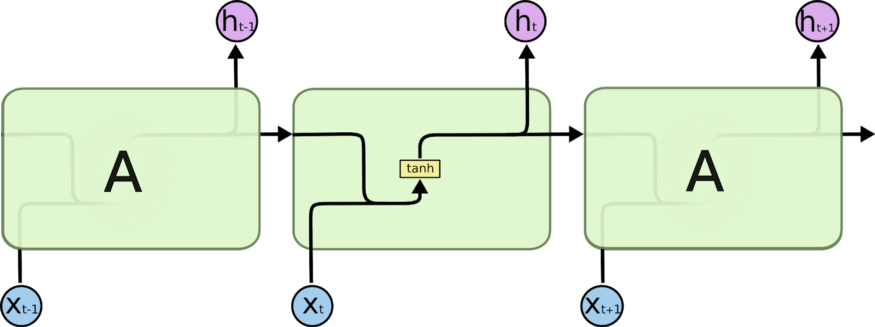
\includegraphics[width=10cm]{figs/RNN.png}
\label{fig:test}
\end{figure}
شبکه‌های عادی پیشرو چیزهایی را که در طول آموزش آموخته اند به خاطر می‌آورند. در حالی که شبکه‌های بازگشتی در حین آموزش به طور مشابه یاد می‌گیرند، علاوه بر این، هنگام تولید خروجی (ها) چیزهایی را که از ورودی‌های قبلی آموخته اند به خاطر می‌آورند. در واقع شبکه‌های بازگشتی حافظه از ورودی قبلی دارند و دنباله ورودی‌ها را متوجه می‌شوند.
\subsection{\trans{مدل توجه}{Attention}}
این مدل
توجه
از دو جهت با مدل کلاسیک متفاوت است.	
در مقایسه با مدل ساده مدل کلاسیک، در اینجا واحد
\trans{رمزگذار}{ٍEncoder}
داده‌های بیشتری را به واحد
\trans{رمزگشا}{Decoder}
منتقل می‌کند. قبلاً تنها، آخرین
\trans{حالت مخفی}{Hidden State}
قسمت رمزگذاری به رمزگشایی ارسال می‌شد، اما اکنون رمزگذار تمام حالت‌های پنهان (حتی حالت‌های میانی) را به رمزگشایی منتقل می‌کند.
قسمت رمزگشایی قبل از تولید خروجی یک مرحله اضافی(در زیر توضیح داده شده) انجام می‌دهد.
آخرین مرحله رمزگشایی به شرح زیر است:
\begin{itemize}
\item هر حالت پنهانی را که دریافت کرده است بررسی می‌کند زیرا هر حالت پنهان رمزگذار بیشتر با کلمه خاصی از جمله ورودی مرتبط است.
\item به هر حالت پنهانی امتیاز می‌دهد.
\item درنهایت هر نمره در نمره softmax مربوط ضرب می‌شود، بنابراین حالتهای پنهان را با امتیاز بالا تقویت می‌کند و حالتهای پنهان را با امتیاز پایین از بین می‌برد.
\end{itemize}

\begin{figure}[H]
\centering
\caption{  معماری مدل مبدل \cite{Ashish2017Attention}}\label{RNN}
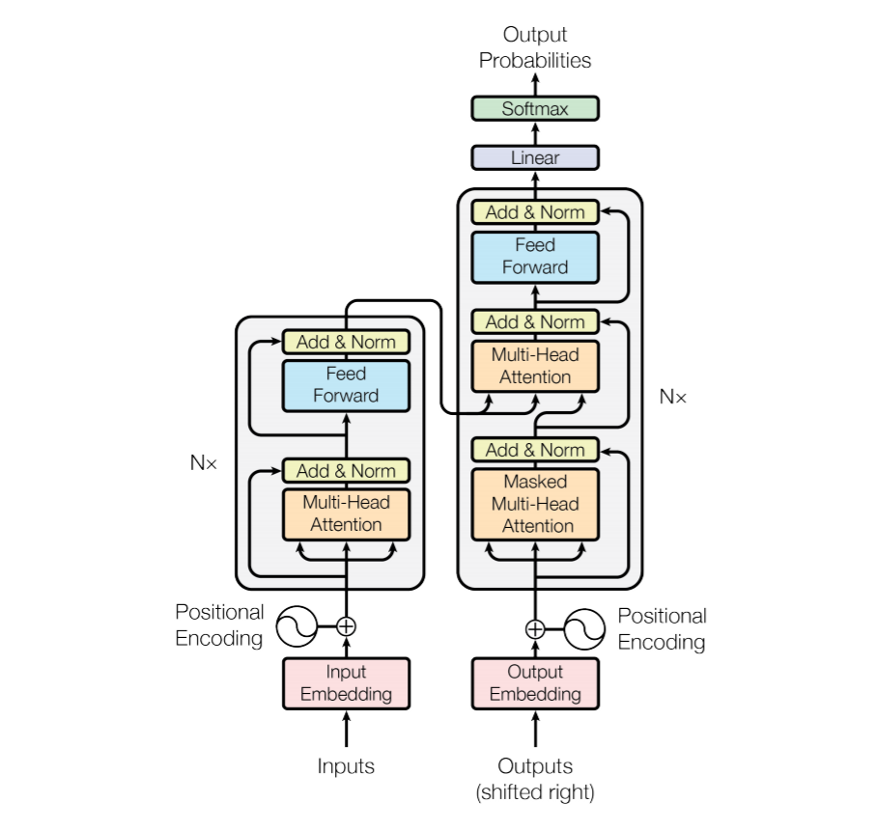
\includegraphics[width=15cm]{figs/Transformer.png}
\label{fig:test}
\end{figure}







\section{\lr{Google BERT}}
\trans{Bert}{Bidirectional Encoder Representations from Transformers}
\cite{Jacob2019Bert}
\cite{RoBERTa}
مقاله ای است که اخیراً توسط محققان \lr{Google AI Language} منتشر شده است، که در بسیاری از مسائل  پردازش زبان طبیعی
\trans{پیشرفته‌ترین}{state-of-the-art}
نتایج را داشت.
مهمترین نوآوری فنی BERT استفاده از آموزش دو طرفه مبدل، در مدل سازی زبان است.
نتایج مقاله نشان می‌دهد که یک مدل زبانی که به صورت دو طرفه آموزش دیده است، می‌تواند نسبت به مدل‌های زبانی تک جهت، حس عمیق تری از موضوع متن و جریان آن زبان داشته باشد.

BERT از مبدل استفاده می‌کندو بر اساس سازوکار توجه  روابط متنی بین کلمات (یا کلمات فرعی) را در یک متن می‌آموزد. در شکل وانیلی، مبدل شامل دو مکانیسم مجزا است - یک رمزگذار که ورودی متن را می‌خواند و یک رمزگشایی که یک پیش بینی برای ورودی تولید می‌کند. از آن‌جا که هدف BERT ایجاد یک مدل زبانی است، فقط مکانیزم رمزگذار لازم است.
Bert از موفقیت بی نظیر در پردازش زبان طبیعی به کمک
\trans{آموزش}{Training}
به کمک 
\trans{مدل سازی ماسک زبان}{Masked-Language Modeling}
(MLM) و
\trans{ پیش بینی جمله بعدی}{Next Sentence Prediction}
(NSP) از موفقیت بی نظیری برخوردار است.
مدل BERT به ما این امکان را می‌دهد که با استفاده از مدل
\trans{ از‌پیش‌آموزش‌داده‌شده}{Pre-trained}
آن را برای مساله‌ی مورد نظر خود 
\trans{تنظیم دقیق}{Fine-tune}
کنیم.

\subsection{توصیف مدل}
Bert یک مدل مبدل است که بر روی یک
\trans{ مجموعه‌نوشته‌ها}{Corpus}
ی
بزرگی از داده‌های چند زبانه
به صورت
\trans{خودنظارتی}{Self-supervised}
پیش‌آموزش می‌شود.
این به این معنی است که فقط بر روی متون خام پیش‌آموزش انجام می‌گیرد، بدون این‌که  توسط انسان برچسب‌گذاری شوند و با یک فرایند خودکار تولید ورودی‌ها و برچسب‌ها انجام می‌شود.
در نگاهی 
دقیق تر، این‌کار با دو هدف مورد توجه قرار می‌گیرد.

\begin{itemize}
\item مدل سازی زبان ماسک :(MLM) با دریافت یک جمله، مدل به طور تصادفی 15٪ از کلمات را در ورودی ماسک می‌کند و سپس کل جمله ماسک را از طریق مدل اجرا کرده و باید کلمات ماسک را پیش بینی کند.تفاوت این مدل با شبکه‌های عصبی بازگشتی که معمولا کلمات را یکی پس از دیگری می‌بینند، این اجازه را می‌دهد تا مدل برای یادگیری، یک نمایش دو طرفه از جمله را بیاموزد.
\item پیش بینی بعدی جمله :(NSP) مدل‌ها دو جمله ماسک را به عنوان ورودی‌ها در طول پیش‌آموزش به هم پیوند می‌زنند. آموزش بر این اساس انجام می‌شود که ایا دو جمله در متن اصلی در کنار یک‌دیگر قرار داشته‌اند یا خیر. داده‌های آموزش نیز بر همین اساس ساخته شده و به عنوان ورودی مدل در نظر گرفته می‌شوند.
\end{itemize}

\subsection{\trans{شهرت نام تجاری}{Net Brand Reputation}}
\trans{رسانه‌های اجتماعی}{Social Media}
، علم و فناوری سطح زندگی مردم و جامعه را افزایش داده است. امروزه رسانه‌های اجتماعی نقش بسیار مهمی‌را با پیشرفت صنایع و شرکت‌ها ایفا می‌کنند. این امر به عنوان یک عامل اساسی توسط شرکت‌ها و هم‌چنین مردم در نظر گرفته شده است. به نحوی که همه مردم به هر طریقی به شبکه‌های اجتماعی متصل هستند. ترکیب فناوری و روابط اجتماعی باعث شده است که افراد بتوانند اطلاعات را با یک‌دیگر به اشتراک بگذارند. رسانه‌های اجتماعی در ده سال گذشته به عنوان یک بستر غالب برای به اشتراک گذاری اطلاعات ظاهر شده است. تجزیه و تحلیل احساسات به کاربر این امکان را می‌دهد تا احساسات، اعتقادات و دیدگاه‌ها را در جهان بزرگ‌تر نشان دهد. علم و فناوری کامپیوتر به اما این امکان را می‌دهد تا بتوانیم با دقت نسبتا خوبی تمایل احساسات و نظرات مردم در شبکه‌های اجتماعی را محاسبه کنیم به شکلی که بتوانیم هر متن به اشتراک گذاشته شده را از نظر مثبت یا منفی بودن ارزیابی کنیم.
حال
برای بدست آوردن شهرت نام تجاری یک نشان تجاری سه مرحله داریم.
\begin{itemize}
\item \subsubsection{استخراج پیام‌های مربوط به برند مربوط}  در این مرحله با توجه به نوع تحقیق و پژوهشی که در حال انجام است، اولین نیاز برای محاسبه شهرت نام تجاری یک برند استخراج پیام‌هایی است که مردم در یک یا چند رسانه اجتماعی به اشتراک گذاشته‌اند. در اینجا تمامی‌تحلیل‌های ما بر روی متن پیام‌هاست.
\item \subsubsection{محاسبه تمایل هر پیام مربوط} در این مرحله به کمک مدل‌های شبکه‌عصبی آموزش‌داده‌شده می‌توانیم تمایل هر پیام استخراج شده مربوط به نشان تجاری مورد نظر را بدست آوریم. به طوری که به هر پیام بر اساس بار معنایی به هر پیام یک برچسب  پیش‌بینی مثبت یا منفی می‌زنیم.
\item \subsubsection{محاسبه شهرت نام تجاری یک نشان تجاری} در این مرحله بعد از بدست آوردن پیام‌های مربوط به برند مورد نظر به همراه برچسب‌های مثبت یا منفی به معنای بار احساسات آن‌ها، معیاری تعریف می‌کنیم که عددی بین -1 و +1 به ما بدهد (+1 به معنای شهرت مثبت بالا و -1 به معنای شهرت   منفی بالا) و آن را عدد شهرت نام تجاری نشان تجاری مورد نظرمان می‌نامیم. این رابطه به شکل زیر است. \\ \begin{equation}
NBR= \dfrac{\#Positive -\#Negative}{\#Positive + \#Negative}
\end{equation}
\end{itemize}
همانطور که در رابطه 2-1 می‌بینیم تعداد پیام‌های با بارمثبت منهای تعداد پیام‌های با بار منفی شده و سپس بر جمع آن‌ها تقسیم شده است. معیار بدست آمده  را شهرت نام تجاری برندی درنظر می‌گیریم که پیام‌های استخراج شده مربوط به آن اند.

\\

\section{ParsBert}

ParsBERT \cite{Mehrdad2020ParsBERT} 
‌مدلی تک زبانه برای Bert در ‌زبان فارسی پیشنهاد می‌کند که عملکرد برتر را در مقایسه با معماری‌ها و مدل‌های چند زبانه دارد. همچنین، از آنجا که میزان داده‌های موجود برای وظایف پردازش زبان طبیعی به زبان فارسی بسیار محدود است، یک مجموعه داده عظیم برای کارهای مختلف پردازش زبان طبیعی و همچنین پیش آموزش این مدل جمع‌آوری شده است. ParsBERT نتایج بهتری را در همه مجموعه‌دادگان نسبت به BERT چند زبانه و سایر کارهای قبلی در تجزیه و تحلیل احساسات و دسته بندی متن بدست‌آورده‌است.


\section{DeepSentiPers}
در این مدل
\cite{Javad2020DeepSentiPers}
ترکیبی از شبکه 
LSTM 
\cite{Sepp1997LSTM}
\cite{Dimensional}
و 
شبکه
CNN
\cite{lecun1989handwritten}
\cite{lecun2015deep}
برای دسته‌بندی جملات ارائه می‌شود.

دستاورد اصلی مجموعه‌های یادگیری عمیق پیشنهادی هر دو نمرات f1 مناسب را کسب کرده اند.  اما، B-LSTM به دلیل واحدهای حافظه داخلی که قادر به کنترل وابستگی‌های طولانی مدت هستند، برای طبقه‌بندی احساسات بهتر عمل می‌کند.  تحقیقات همچنین این ایده را تأیید می‌کند که معماری CNN برای محدوده پردازش تصویر مناسب است نه طبقه‌بندی متن.  بنابراین، تحقیقات بیشتری می‌توان در LSTM دو طرفه در ارتباط با تجزیه و تحلیل احساسات انجام داد.


\قسمت{جمع‌بندی}

با توجه به دو بخش آخر این فصل و بیان مزایا و معایب هر کدام از مدل‌های 
\lr{DeepSentiPers}
و 
\lr{ParsBert}
و هم‌چنین تحقیق در مورد آن‌ها ما از مدل 
\lr{ParsBert}
استفاده کرده و آن را تا حد بسیار زیادی بهبود داده‌ایم.